%% LaTeX Beamer presentation template (requires beamer package)
%% see http://latex-beamer.sourceforge.net/
%% idea contributed by H. Turgut Uyar
%% template based on a template by Till Tantau
%% this template is still evolving - it might differ in future releases!

\documentclass{beamer}
\usepackage[utf8]{inputenc}
\usepackage{etex}

%http://www.informatik.uni-freiburg.de/~frank/latex-kurs/latex-kurs-3/Latex-Kurs-3.html
\usepackage{beamerthemeshadow}
\beamersetuncovermixins{\opaqueness<1>{25}}{\opaqueness<2->{15}}
% \mode<presentation>
% {
% \usetheme{Boadilla}
% %\usetheme{Dresden}
% %\usetheme{Madrid}
% %\usetheme{Singapore}
% 
% \usecolortheme{wolverine}
% %\usecolortheme{crane}
% %\usecolortheme{dove}
% %\usecolortheme{seagull}
% %\usecolortheme{seahorse}
% %\usecolortheme{rose}
% 
% \setbeamerfont{title}{shape=\itshape,family=\rmfamily}
% %\setbeamercolor{title}{fg=red!80!black}
% %\setbeamercolor{title}{fg=red!80!black,bg=red!20!white}
% 
% \usefonttheme{serif}
% %\usefonttheme{structuresmallcapsserif}
% 
% \setbeamercovered{transparent}
% }


\usepackage[english]{babel}
\usepackage{babelbib}

% font definitions, try \usepackage{ae} instead of the following
% three lines if you don't like this look
\usepackage{mathptmx}
\usepackage[scaled=.90]{helvet}
\usepackage{courier}


\usepackage[T1]{fontenc}
\usepackage{pictex}
\usepackage{dsfont}
\usepackage{ulem}


\title{ESE CPCC Project}

%\subtitle{}

% - Use the \inst{?} command only if the authors have different
%   affiliation.
%\author{F.~Author\inst{1} \and S.~Another\inst{2}}
\author[M. Kleber, C. Krainer, A. Schr\"ocker, B. Zechmeister]{Michael Kleber, Clemes Krainer,\\ Andreas Schr\"ocker, Bernhard Zechmeister}

% - Use the \inst command only if there are several affiliations.
% - Keep it simple, no one is interested in your street address.
\institute[University of Salzburg]
{
% \inst{1}%
Department of Computer Sciences\\
  University of Salzburg, Austria
% \and
% \inst{2}%
% Department of Theoretical Philosophy\\
% Univ of E
}

\date{\today}


% This is only inserted into the PDF information catalog. Can be left
% out.
\subject{Talks}



% If you have a file called "university-logo-filename.xxx", where xxx
% is a graphic format that can be processed by latex or pdflatex,
% resp., then you can add a logo as follows:

% \pgfdeclareimage[height=0.5cm]{university-logo}{university-logo-filename}
% \logo{\pgfuseimage{university-logo}}



% Delete this, if you do not want the table of contents to pop up at
% the beginning of each subsection:
\AtBeginSubsection[]
{
\begin{frame}<beamer>
	\frametitle{Outline}
	\tableofcontents[currentsection,currentsubsection]
\end{frame}
}

% If you wish to uncover everything in a step-wise fashion, uncomment
% the following command:

%\beamerdefaultoverlayspecification{<+->}

\begin{document}

\begin{frame}
	\titlepage
\end{frame}

\begin{frame}
	\frametitle{Content}
	\tableofcontents
% You might wish to add the option [pausesections]
\end{frame}


% - Einleitung
%   - Aufgabenstellung
%   - Systemarchitektur: Pilot, Engine, Mapper, GMView, Planner, ...
%   - Datenaustausch mit HTTP(S)
\section{Introduction}
%\subsection[Short First Subsection Name]{First Subsection Name}

\subsection{Project Description}

\begin{frame}\frametitle{Introduction}\framesubtitle{Task}
	\begin{itemize}
		\item simulation of physical helicopter swarms
		\item simulation of sensors
		\item abstraction of virtual vehicles (virtual helicopters)
		\item migration of virtual vehicles among flying physical helicopters
	\end{itemize} 
\end{frame}

\begin{frame}\frametitle{Introduction}\framesubtitle{Project Scope}
	\begin{itemize}
		\item real vehicles (physical helicopters) follow strict flight plans
		\item no network bandwith limits
		\item no processing power limits
	\end{itemize} 
\end{frame}

\begin{frame}\frametitle{Introduction}\framesubtitle{Applied Technologies}
	\begin{itemize}
		\item HTTP as protocol for sensor abstraction and data exchange
		\item Java as programming language
		\item software implemented as web applications
		\item Apache Tomcat as web server and servlet container
	\end{itemize} 
\end{frame}

\subsection{System Overview}

\begin{frame}\frametitle{Introduction}\framesubtitle{System Overview}
	\begin{center}
		{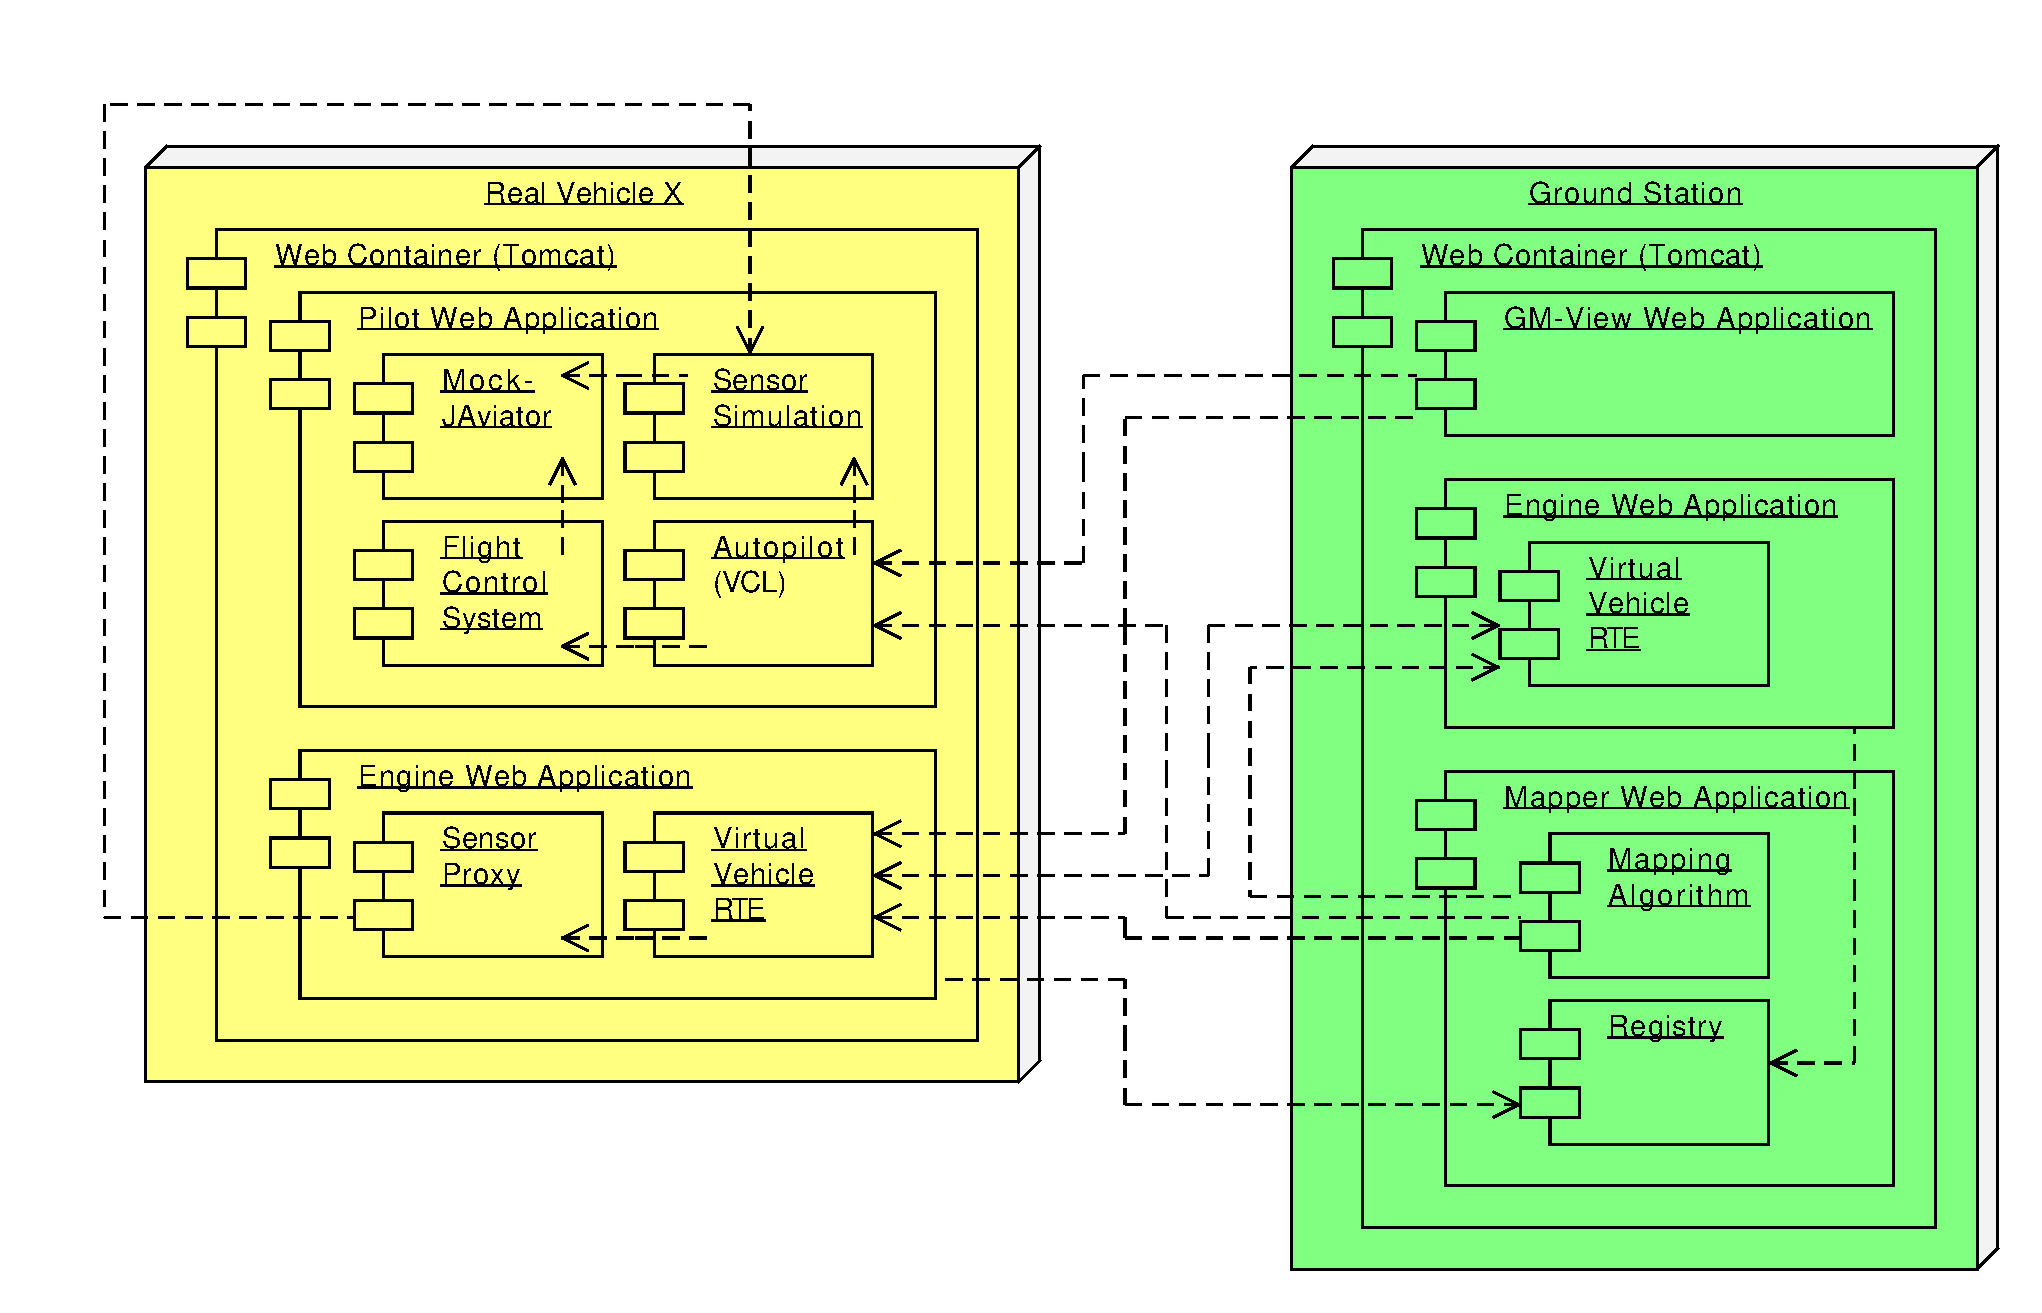
\includegraphics[width=10cm]{SystemOverview.pdf}}
	\end{center}
\end{frame}

\begin{frame}\frametitle{Introduction}\framesubtitle{Sensor Simulation}
	\begin{center}
		{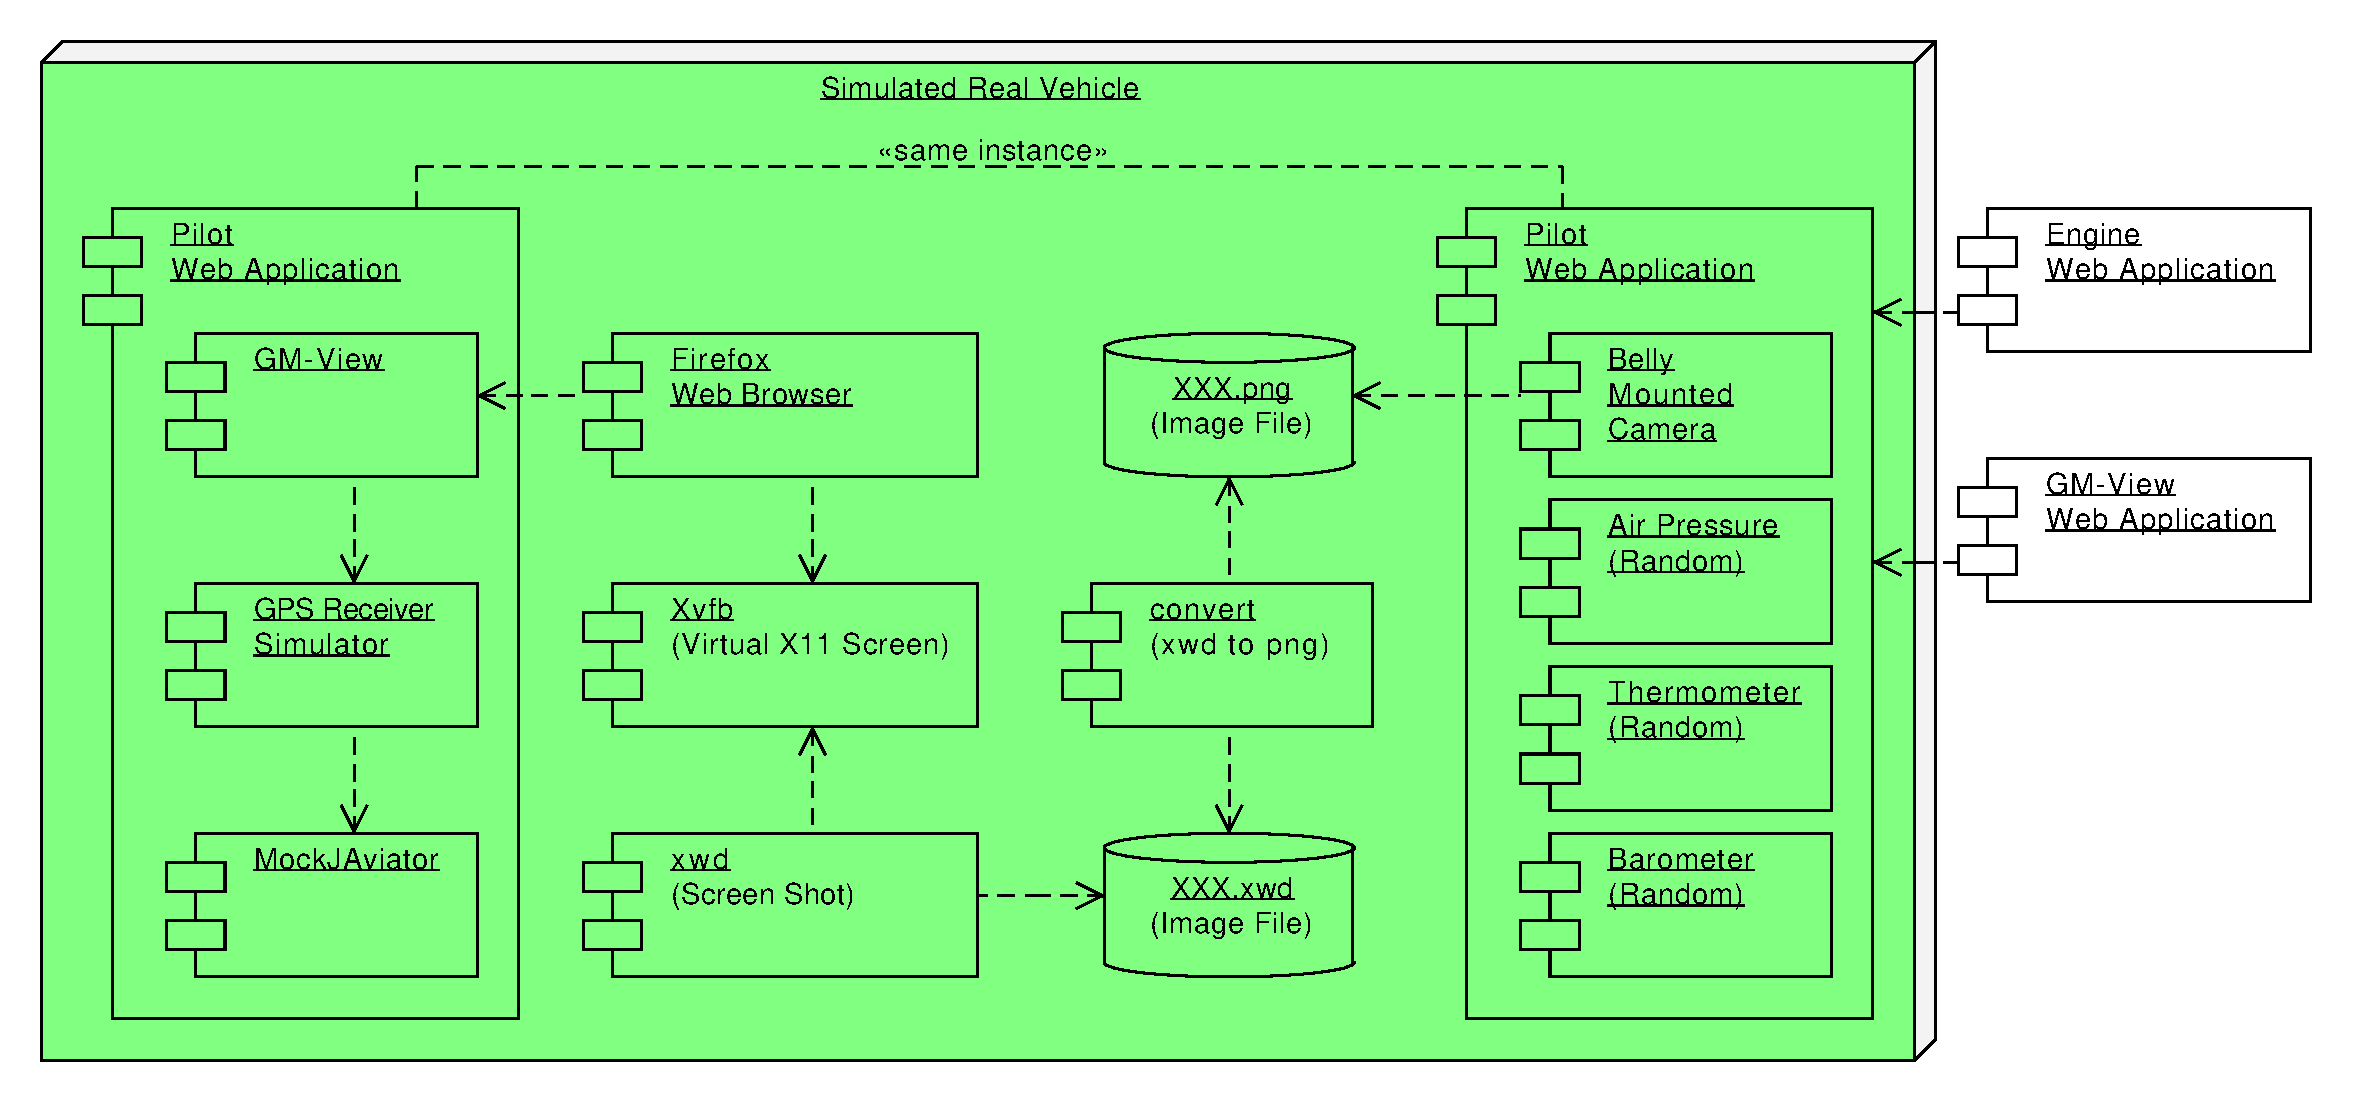
\includegraphics[width=11cm]{SensorSimulation-2.pdf}}
	\end{center}
\end{frame}

\section {Implementation}

% - Real Vehicles
%   - Flugplan / VCL
%   - Simulation
%   - Sensoren
\subsection{Real Vehicles}

\begin{frame}\frametitle{Real Vehicles}\framesubtitle{Vehicle Configuration}
plant.simulated = true \\
plant.type = MockJAviator \\
plant.listener = udp://localhost:9011 \\
plant.location.system.type = gpssim \\
plant.location.system.listener = tcp://localhost:9012 \\
plant.location.system.update.rate = 10 \\
 \\
controller.simulated = true \\
controller.type = JControl \\
 \\
pilot.type = JPilot \\
pilot.name = Pilot One \\
pilot.controller.connector = udp://localhost:9014
\end{frame}


\begin{frame}\frametitle{Real Vehicles}\framesubtitle{Sensor Configuration}
sensor.list = gps, temp, photo \\
\\
sensor.gps.name = GPS receiver \\
sensor.gps.path = position \\
sensor.gps.uri = gps:/// \\
\\
sensor.temp.name = thermometer \\
sensor.temp.path = temperature \\
sensor.temp.uri = rand:///18/22 \\
\\
sensor.photo.name = belly mounted photo camera \\
sensor.photo.path = photo \\
sensor.photo.uri = x11:///:21
\end{frame}


\begin{frame}\frametitle{Real Vehicles}\framesubtitle{Vehicle Control Language}
\#\# \\
\#\# @(\#) real vehicle set course \\
\#\# \\
go auto \\
takeoff 1m for 5s \\
fly to (47.82204197, 13.04086670, 20.00)abs precision 1m 2.0mps \\
fly to (47.82206088, 13.04092035, 20.00)abs precision 1m 2.0mps \\
fly to (47.82195102, 13.04488063, 20.00)abs precision 1m 2.0mps \\
hover for 20s \\
land \\
go manual
\end{frame}


% - Vehicle Virtualisierung
%   - Prinzipielle Funktion eines VV-Programms
%   - Status / Serialisierung / Migration
%   - VV-Language: Command = Point + Actions
%   - Scanner, Parser
\subsection{Vehicle Virtualization}

\begin{frame}\frametitle{Vehicle Virtualization}\framesubtitle{Virtual Vehicle Program}
\begin{itemize}
\item ability to suspend
\item state is serialized
\item information is persisted to file
\item migration can be performed
\item virtual vehicle can resume
\end{itemize} 
\end{frame}

\begin{frame}\frametitle{Vehicle Virtualization}\framesubtitle{Virtual Vehicle Language}
\begin{itemize}
\item list of commands
\item command consits of a point and a list of actions
\item point contains latitude, longitude, altitude
\item specification of tolerance
\end{itemize} 
\end{frame}

\begin{frame}\frametitle{Vehicle Virtualization}\framesubtitle{Virtual Vehicle Sample Program}
Point 47.82201946 13.04082647 1.00 tolerance 12.3\\
Picture \\
Temperature\\
\\
Point 47.82203026 13.04084659 25.00 tolerance 100 \\
Temperature\\
\\
Point 47.82211311 13.04076076 30.00 tolerance 1.2\\
Picture
\end{frame}

\begin{frame}\frametitle{Vehicle Virtualization}\framesubtitle{Scanner \& Parser}
\begin{itemize}
\item \ldots
\end{itemize} 
\end{frame}

% - Mapping
%   - Registrierung der Engines
%   - Algorithmen: Random, Simple
%   - Ansto� der Migration
\subsection{Mapping}

\begin{frame}\frametitle{Mapper}
	\begin{itemize}
		\item maps virtual vehicles to real vehicles 
		\item invokes migration
		\item two components:
			\begin{itemize}
				\item registration service
				\item mapper
			\end{itemize}
	\end{itemize} 
\end{frame}

\begin{frame}\frametitle{Mapper}\framesubtitle{Registration Mapper}
	\begin{itemize}
		\item engine registers itself with registration service
		\item service fetches useful information:
		\begin{itemize}
			\item sensors
			\item waypoints
		\end{itemize}
	\end{itemize} 
\end{frame}

\begin{frame}\frametitle{Mapper}\framesubtitle{Mapper}
	\begin{itemize}
		\item periodic
		\item fetches status of all virtual vehicles
		\begin{itemize}
			\item next action point
			\item and its actions
		\end{itemize}
		\item status of all real vehicles
		\begin{itemize}
			\item current position
			\item next position
			\item velocity
		\end{itemize}
		\item two algorithms:
		\begin{itemize}
			\item random mapping algorithm
			\item simple mapping algorithm
		\end{itemize}
	\end{itemize} 
\end{frame}

\begin{frame}\frametitle{Mapper}\framesubtitle{Simple Mapping Algorithm}
	\begin{tabbing}
	\textbf{for} \= \textbf{all} virtual vehicles \textbf{do} \\[.25cm]
	\> \textbf{if}  \= virtual vehicle program is complete \\
	\> \>	\textbf{then} invoke migration to central engine \\[.25cm]
	\>	\textbf{else} \= find fastest real vehicle with at least one needed sensor \\
	\> \>	\textbf{and} distance CN to P < tolerance \\[.25cm]
	\>	\textbf{if} found vehicle \textbf{then} invoke migration to it \\
	\end{tabbing}
\end{frame}

\section{Live Demonstration}
% - Demo 1: "VV sammelt Daten"
%   - Setup: 1xRV, 1xVV, 2xVV-Points
%   - RV fliegt die VV-Points ab
%   - VV sammelt die Daten ein
\subsection{Demo 1 - Data Collection}

\begin{frame}\frametitle{Live Demonstration}\framesubtitle{Demo 1: Data Collection}
% Flying time 00:04:43
	\begin{itemize}
		\item one flying real vehicle
		\item one virtual vehicle that collects data at four locations
		\item no migration
	\end{itemize}
	\vspace{0.5cm}
	\begin{center}
		{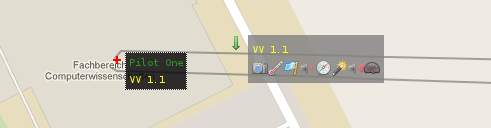
\includegraphics[width=10cm]{demo1.png}}
	\end{center}
\end{frame}

% - Demo 2: "VV wird migriert"
%   - Setup: 2xRV, 1xVV, 2xVV-Points
%   - Je ein RV fliegt einen VV-Point an
%   - VV sammelt am RV1 die ersten VV-Point Daten
%     ein, wird migriert und macht am RV2 weiter.
\subsection{Demo 2 - Virtual Vehicle Migration}

\begin{frame}\frametitle{Live Demonstration}\framesubtitle{Demo 2: Virtual Vehicle Migration}
% Flying time 00:05:55
	\begin{itemize}
		\item two flying real vehicles
		\item one virtual vehicle that collects data at five locations
		\item migration among both real vehicles
	\end{itemize}
	\vspace{0.5cm}
	\begin{center}
		{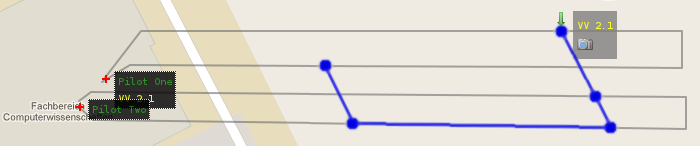
\includegraphics[width=10cm]{demo2.png}}
	\end{center}
\end{frame}

% - Demo 3: "RVs haben unterschiedliche Sensoren"
%   - Setup: 3xRV, 1xVV, 1xVV-Point
%   - Alle RVs fliegen nacheinander einen VV-Point an
%   - VV sammelt am RV1 die ersten VV-Point Daten
%     ein, wird migriert auf RV2, sammelt weiter Daten
%     ein, wird migriert auf RV3 und sammelt die
%     restlichen Daten ein.
\subsection{Demo 3 - Real Vehicles with different Sensors}

\begin{frame}\frametitle{Live Demonstration}\framesubtitle{Demo 3: Real Vehicles with different Sensors}
	\begin{itemize}
		\item three flying real vehicles carrying different sensors
		\item one virtual vehicle that collects data at two locations
		\item migration among all real vehicles
	\end{itemize}
	\vspace{0.5cm}
	\begin{center}
		{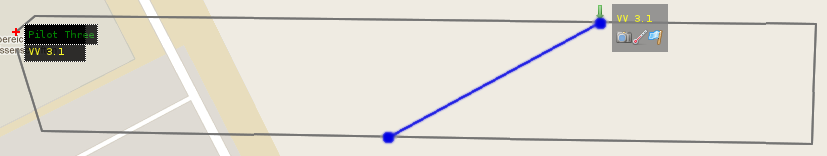
\includegraphics[width=10cm]{demo3.png}}
	\end{center}
\end{frame}


% - Demo 4: "All in one."
%   - Setup: 3xRV, 3xVV, 9xVV-Point
%   - ...
\subsection{Demo 4 - Complex Scenario}

\begin{frame}\frametitle{Live Demonstration}\framesubtitle{Demo 4: Complex Scenario}
	\begin{columns}
		\begin{column}{5cm}
		\begin{itemize}
			\item three flying real vehicles
			\item four virtual vehicle that collect data
			\item migration among all real vehicles
		\end{itemize}
		\end{column}
		\begin{column}{8cm}
		\begin{center}
			{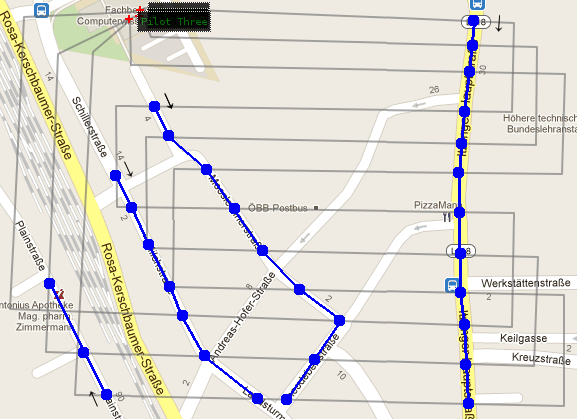
\includegraphics[width=7.7cm]{demo4.png}}
		\end{center}
		\end{column}
	\end{columns}
\end{frame}

% - Future Work
%   - Aufw�ndigere Mapping-Algorithmen
%   - Optimierung Netzwerkverkehr
%   - Video-Sensor
%   - Geo-Location: Vergleich RV-Position zu VV-Sollwert
%   - RV-Flugpl�ne aus VV-Programmen zusammenstellen
\section{Conclusion}

\subsection{Future Work}

\begin{frame}\frametitle{Future Work} %\framesubtitle{xxx}
	\begin{itemize}
		\item more subtle mapping algorithms
		\item network traffic optimizations
		\item video sensor support
		\item extended geo-location
		\item flight plan generation based on virtual vehicle programs
	\end{itemize}
\end{frame}
 

% - Q & A Session
\subsection{Questions and Answers}

\begin{frame}
	\frametitle<presentation>{Questions \& Answers}
	\framesubtitle{~}
	\begin{center}
		\fontsize{64}{64}\selectfont
		\begin{tabular}{ccc}
			Q &&\\
			& ~~\& & \\
			&&~~ A
		\end{tabular}
	\end{center}
\end{frame}

\end{document}
